\documentclass[aspectratio=169]{beamer}              % only frames

% for themes, etc.
\mode<presentation>
\usetheme{Madrid} 
\usecolortheme{crane}

%\usepackage{times}  % fonts are up to you
% The usual suspects
\usepackage{multirow, booktabs, dcolumn, color, graphicx} % Tables\usepackage{graphicx}
\usepackage{amsmath,amssymb,amsthm}
% Strikethrough text
\usepackage{soul}
% Adjust box to fit tabulars
\usepackage{adjustbox}
% Embed video
\usepackage{media9}
% For notes
\usepackage{pgfpages}
%\setbeameroption{hide notes} % Only slides
%\setbeameroption{show only notes} % Only notes
\setbeameroption{show notes on second screen=right} % Both
% Give a slight yellow tint to the notes page
%\setbeamertemplate{note page}{\pagecolor{yellow!5}\insertnote}\usepackage{palatino}
% Use colors by name
\usepackage{xcolor}
% EMBEDDING VIDEO IS POSSIBLE WITH PDFPC USE PDF PC to present
\usepackage{multimedia}



% The table highlighting for hypothesis discussion.
\usepackage[beamer,customcolors]{hf-tikz}
\usetikzlibrary{calc}

% To use background images
\newenvironment{colorframe}[2][]{%
\setbeamercolor{background canvas}{bg=#1}
\begin{frame}\color{white}}
{\end{frame}}


% To set the hypothesis highlighting boxes red.
\tikzset{hl/.style={
    set fill color=red!80!black!40,
    set border color=red!80!black,
  },
}

% Set Graphics folder
\graphicspath{{./figures/}}


% these will be used later in the title page
\title{Common Threats and Solutions}
\subtitle{Password Managers}
\author{Irfan Kanat}
\institute[CBS]{{Department of Digitization}\\ Copenhagen Business School}
\date{\today}



\begin{document}

% this prints title, author etc. info from above
\begin{frame}

	\titlepage

	\vfill
	{\tiny \centering This work is licensed under a \href{http://creativecommons.org/licenses/by/4.0/}{Creative Commons Attribution 4.0 International License}.}

\end{frame}

\note{In this video we will learn how to use a password manager.}

\begin{frame}
	\frametitle{A Strong Password}
    
	Possibilities... \vspace{1em}

	\pause $l = {a b c . . . x y z} = 26 \vspace{1em}$

	\pause $lll = 26 \times 26 \times 26 = 17576 \vspace{1em}$

	\pause $llll = 26 \times 26 \times 26 \times 26 = 456976 \vspace{1em}$	

	\pause $L = {a b c . . . z A B . . . X Y Z} = 52 \vspace{1em}$	

	\pause $LLL = 52 \times 52 \times 52 = 140608 \vspace{1em}$

	\pause Upper, lower case characters, numbers, special symbols...

\end{frame}

\note{The strength of the password can be estimated by how many possible tries it would take to guess the password. This is what a computer trying to \textbf{bruteforce} the password.

So two ways to increase the strength of the password. Size of the character set, and digits. So longer passwords made up of different types of characters (letters, numbers, symbols) are harder than shorter passwords made up of just one type of character.

Bruteforce is not the only way to crack a password. Trying all words in a dictionary, and combinations of words has also been done in the past. This is known as a \textbf{dictionary attack}. So don't use words in your password.

You can also just guess the password by using information about the person. So don't use personal facts as password.
}


\begin{frame}
	\frametitle{Have You Been Pwned?}
    
	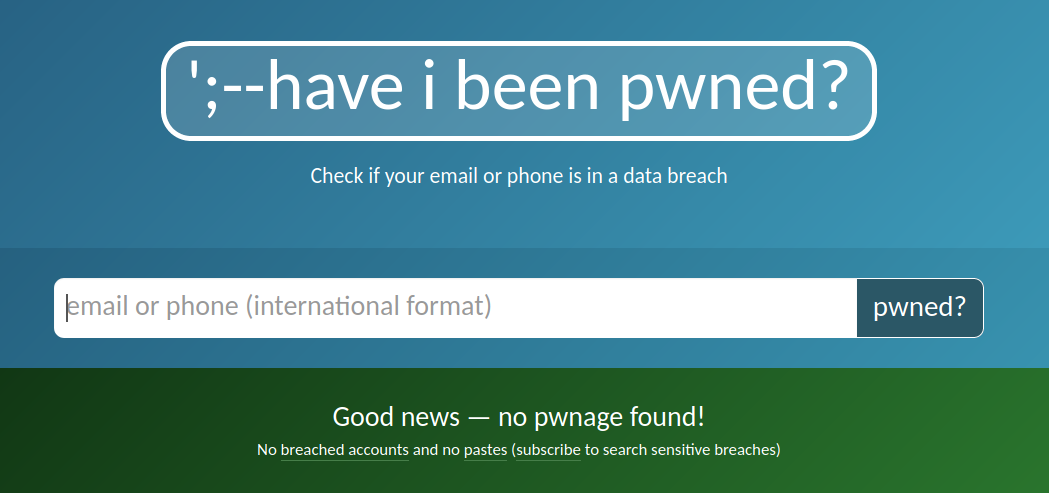
\includegraphics[width = \textwidth, height = .85\textheight, keepaspectratio]{figures/haveIbeenPwned.png}

\end{frame}

\note{One way adversaries may get access to your accounts is by using your known passwords on other accounts.

So if your password was revealed in a data breach, all your other accounts using the same password is also in danger.

I highly recommend you go and check your e-mail address on \url{haveibeenpwned.com}}

\begin{frame}
	\frametitle{Good Password}
    
    Long \vspace{1em}

    Character Types \vspace{1em}

    No Words \vspace{1em}

    No Personal Facts \vspace{1em}

    Don't Reuse	\vspace{1em}

\end{frame}

\begin{frame}
	\frametitle{Password Managers}
    \centering
    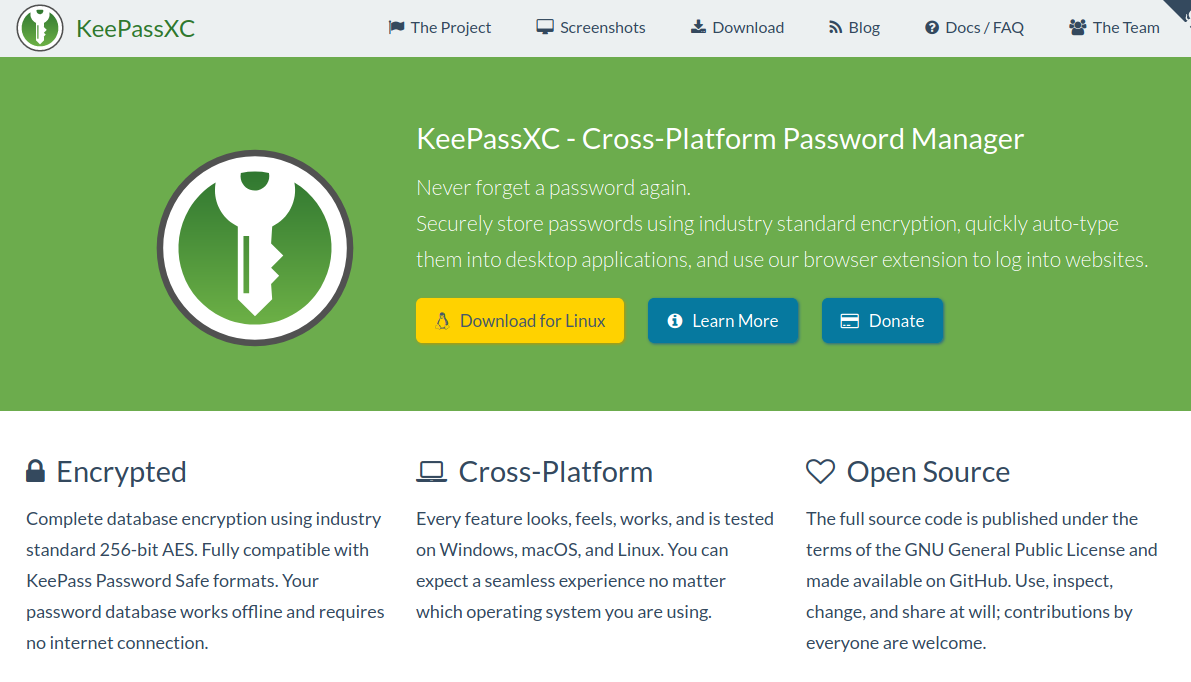
\includegraphics[width = \textwidth, height = .85\textheight, keepaspectratio]{figures/KeepassXC.png}

\end{frame}

\note{A good password is not only hard to guess, it is also hard to remember for humans. So it is imperative you use a password manager.

There are various password managers out there. The most convenient ones are cloud based services like lastpass or 1password. Unfortunately these type of services run the risk of becoming paid after the fact. Last pass for example changed the terms of its free tier in 2020, putting their users in a difficult situation.

Therefore I recommend open source solutions. They are not as convenient, but it gives you more control.}

\end{document}
